\chapter[Conservation applications]{Applications of Species Distribution Models in Conservation}

\begin{objetivos}
By the end of this chapter, readers should be able to explain how SDMs can inform conservation decisions; combine contemporary suitability, future climatic stability, uncertainty indicators, and protected-area coverage; identify candidate priority areas for \textit{Dinizia excelsa}; assess representation and protection gaps; construct transparent spatial-priority indices; and discuss applications to threatened species, giant trees, ecological restoration, monitoring, and systematic conservation planning.
\end{objetivos}

\section{Introduction}

Species distribution models are widely used to support conservation under climate change, habitat loss, forest fragmentation, and expanding human pressure. Their role is not merely to map where a species could find suitable environmental conditions. Conservation decisions also require information about persistence, threats, connectivity, representation, feasibility, costs, governance, and uncertainty \parencite{margules2000systematic,moilanen2009spatial,franklin2023,guisan2017habitat,zurell2020benchmarking}.

This chapter integrates products developed previously into an applied analysis for \textit{Dinizia excelsa}. The resulting maps synthesize ecological and climatic evidence for screening candidate areas. They are decision-support products, not automatic prescriptions for reserve designation or intervention.

\begin{conceito}[title={\faBook\quad SDM as conservation evidence}]
In conservation, an SDM is one spatial layer of evidence. It should be combined with protected-area status, habitat condition, connectivity, exposure to threats, uncertainty, ecological feasibility, management objectives, costs, and the rights and knowledge of affected communities.
\end{conceito}

\section{Defining the decision problem}

Before combining maps, specify the conservation objective, spatial units, planning horizon, target, and decision constraints. Protecting extant populations, restoring habitat, maintaining climatic refuges, establishing corridors, guiding surveys, and supporting assisted migration are different problems and may produce different rankings.

The didactic index in this chapter uses five criteria:

\begin{itemize}
\item high contemporary modeled suitability;
\item persistence of suitability across specified future projections;
\item modeled paleoclimatic stability;
\item a low integrated caution index;
\item representation inside or outside existing protected areas.
\end{itemize}

Protected-area overlap can serve two opposing objectives. Areas inside the network may be priorities for reinforcing management of already represented habitat, whereas suitable areas outside it may reveal representation gaps. The role of this criterion must therefore be defined before scoring.

\begin{atencao}[title={\faExclamationTriangle\quad Suitability alone does not define priority}]
A highly suitable cell may be degraded, disconnected, legally unavailable, environmentally extrapolative, or too costly to manage. Conversely, a moderately suitable cell may be essential for complementarity or connectivity. Prioritization must follow an explicit decision objective rather than a suitability ranking alone.
\end{atencao}

\section{Preparing spatial evidence}

\rscriptfile{scripts/unidade17/01_estrutura_pastas.R}

\rscriptfile{scripts/unidade17/02_preparar_camadas_conservacao.R}

All layers must share a coordinate reference system, extent, resolution, cell origin, and mask. Area calculations should use an equal-area projection or cell-area weighting. Protected-area data require a documented version and date because boundaries, legal categories, and management status can change. Overlap between polygons and raster cells should not be interpreted as effective protection without information on implementation and condition.

\section{Contemporary climatic priority}

\rscriptfile{scripts/unidade17/03_prioridade_climatica_atual.R}

\begin{figure}[H]
\centering
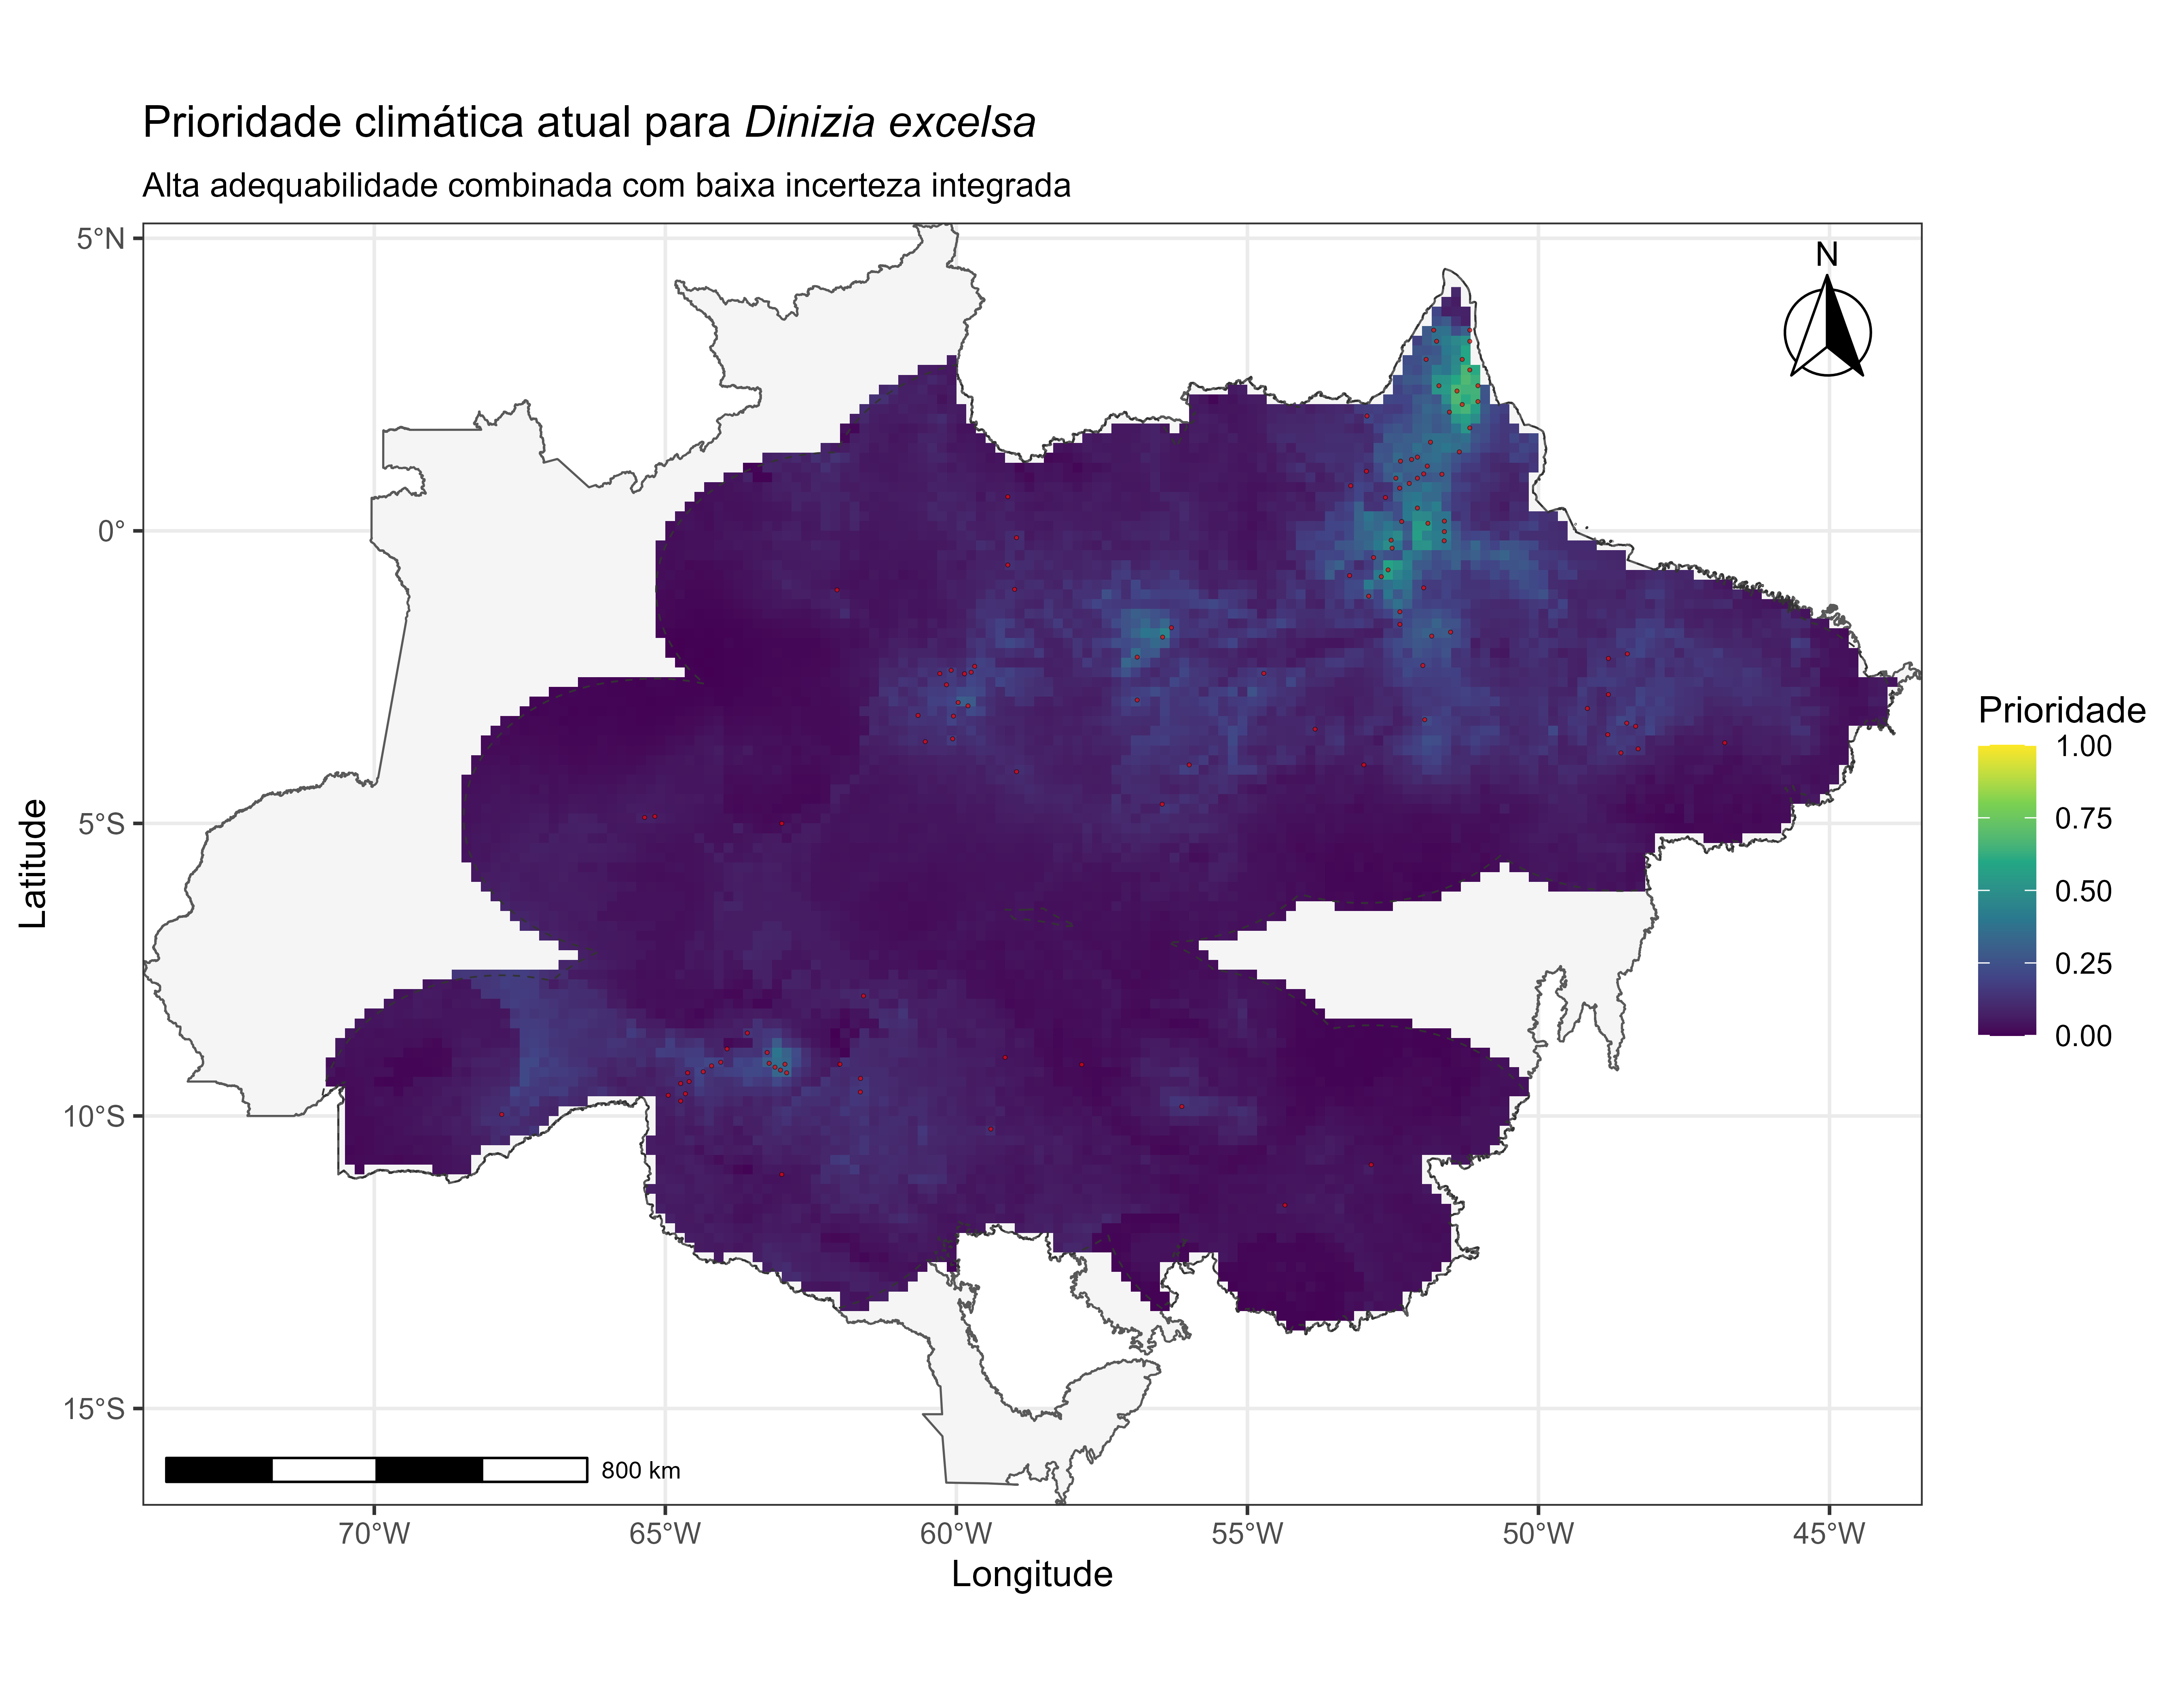
\includegraphics[width=0.88\textwidth]{figuras/unidade17/unidade17_prioridade_climatica_atual.png}
\caption{Contemporary climatic-priority index for \textit{Dinizia excelsa}, based on modeled suitability and the integrated uncertainty indicator.}
\label{fig:unidade17_prioridade_atual}
\end{figure}

This layer identifies locations where the model estimates relatively suitable contemporary conditions with comparatively strong support. It does not confirm population presence, habitat integrity, abundance, regeneration, or demographic viability. Field records and remotely sensed habitat condition should be used to validate candidate sites.

\section{Future stability and conservation}

\rscriptfile{scripts/unidade17/04_estabilidade_futura_conservacao.R}

\begin{figure}[H]
\centering
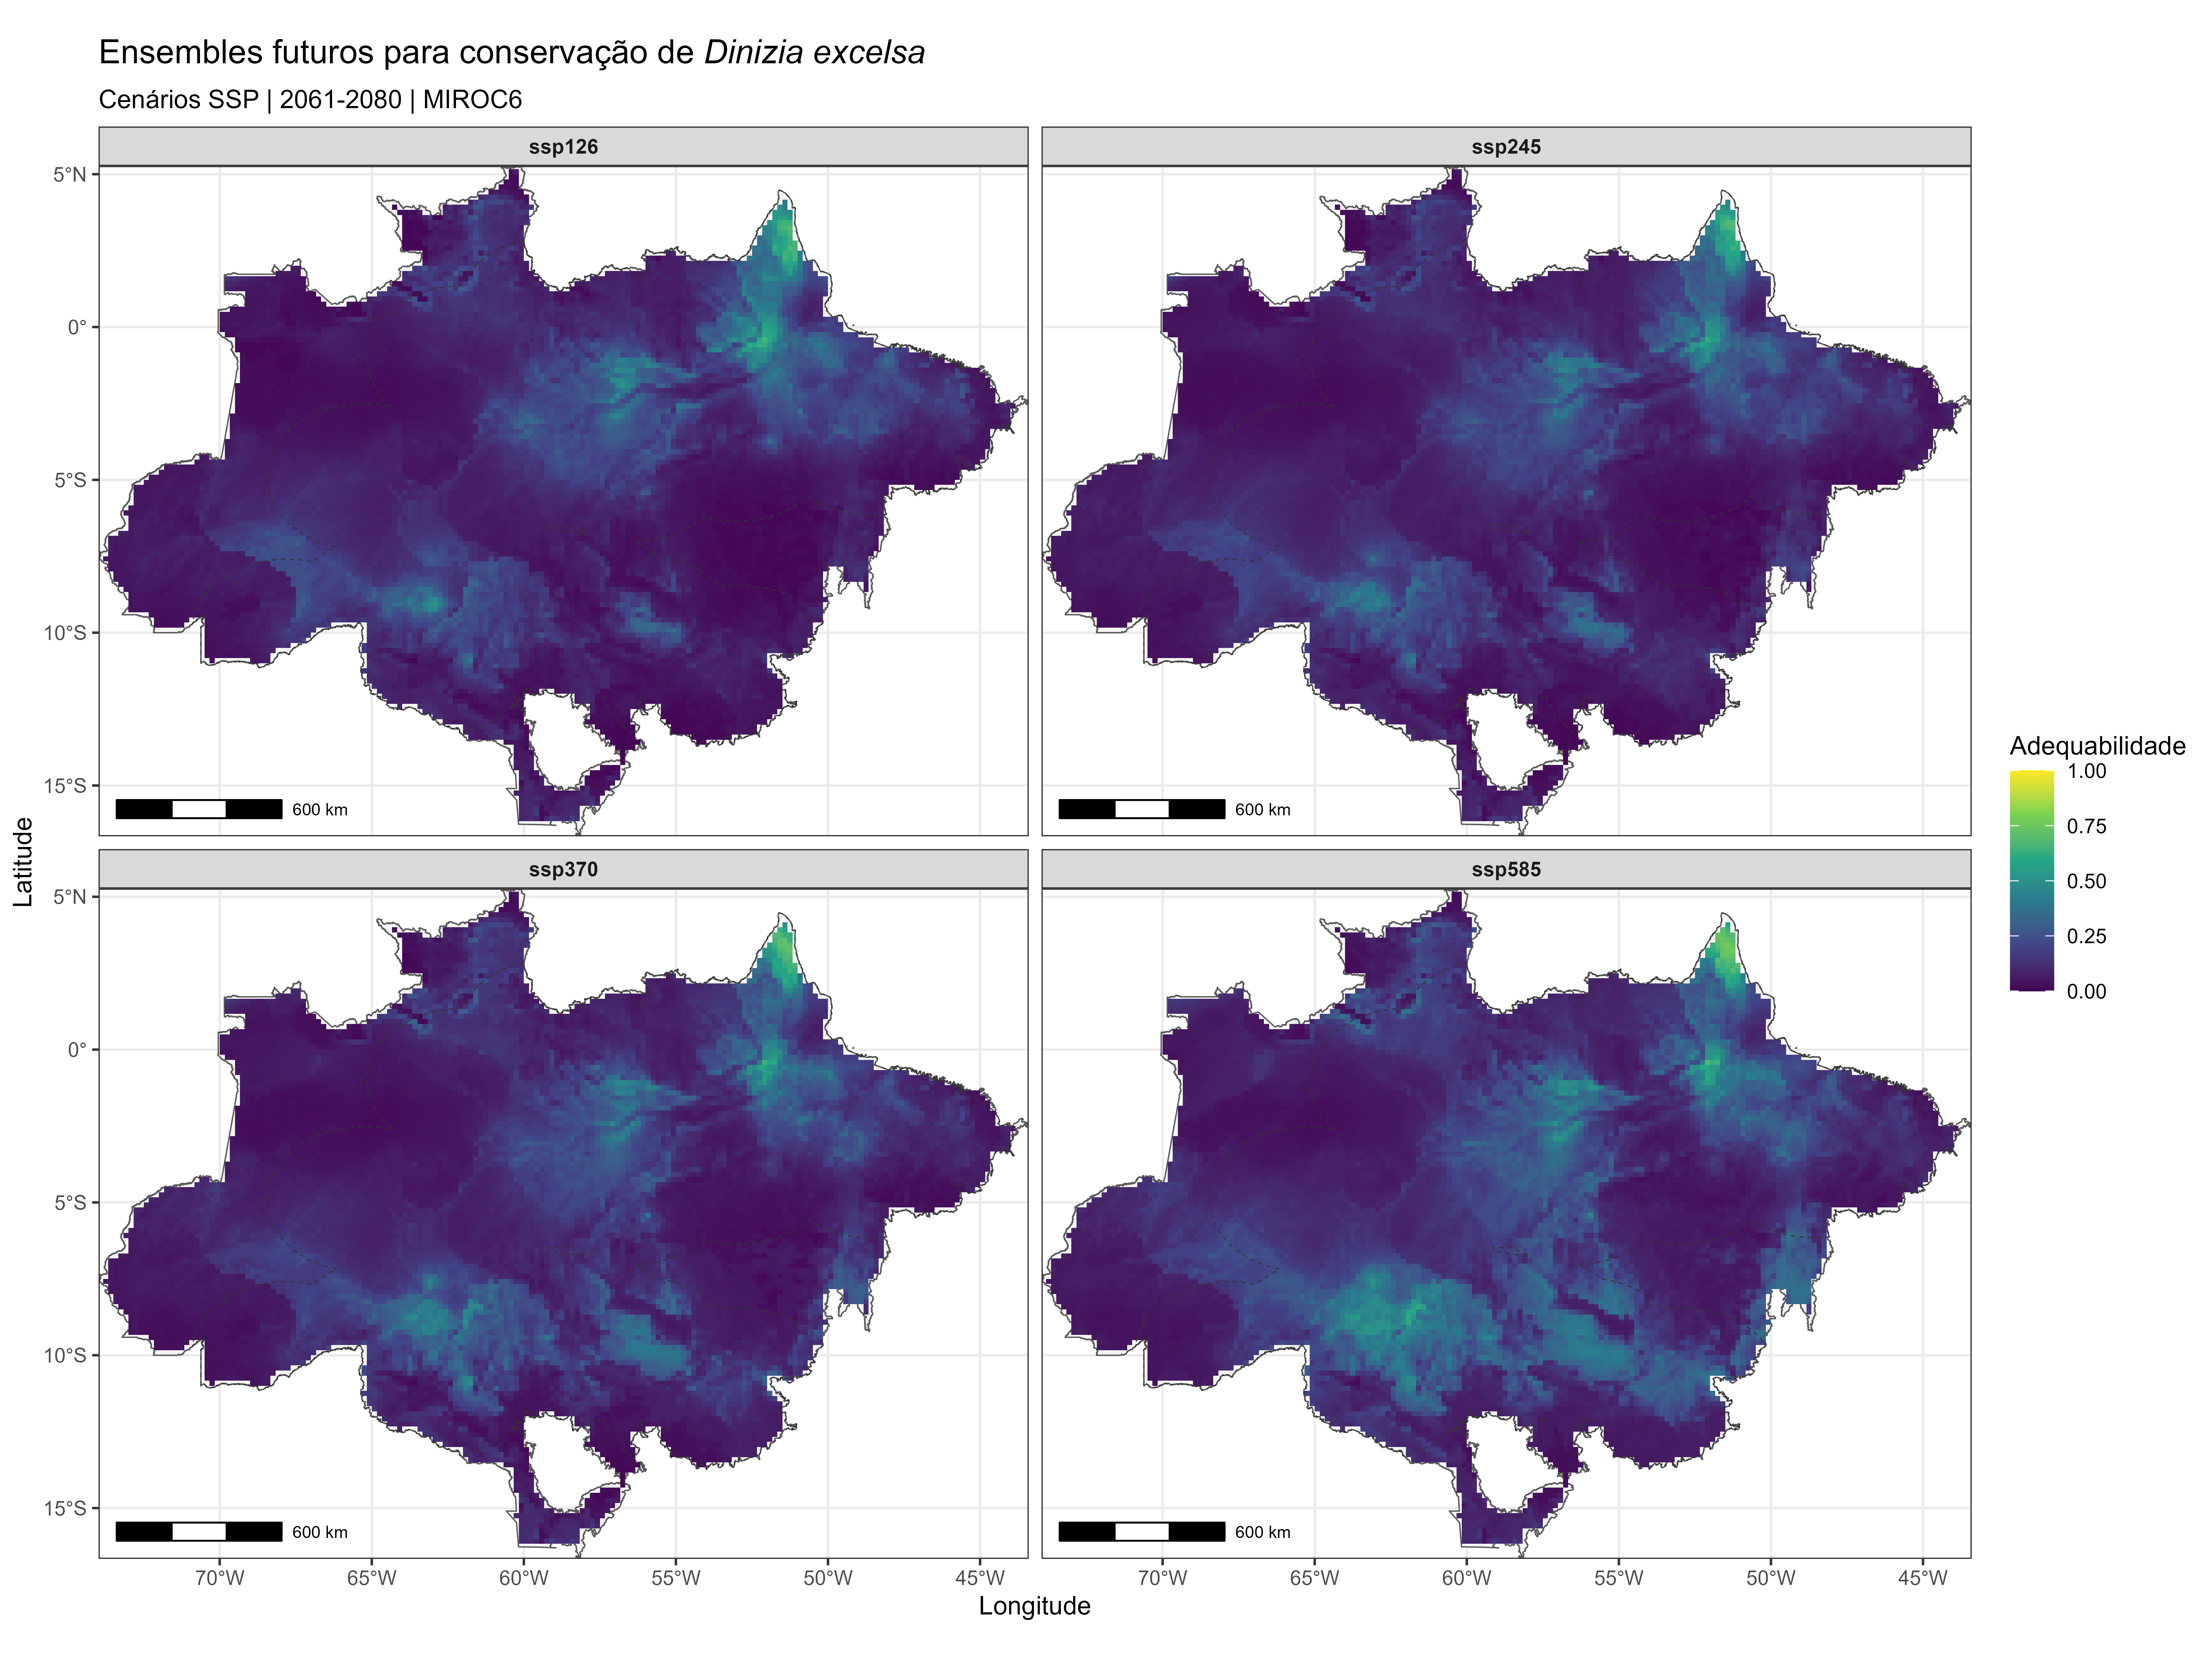
\includegraphics[width=0.96\textwidth]{figuras/unidade17/unidade17_estabilidade_futura_conservacao.png}
\caption{Persistence of projected environmental suitability for \textit{Dinizia excelsa} across specified future climate scenarios.}
\label{fig:unidade17_estabilidade_futura}
\end{figure}

Future stability is conditional on the GCMs, SSPs, time horizons, thresholds, algorithms, and assumptions selected. Requiring agreement across all scenarios is conservative but may discard areas valuable under most futures; averaging scenarios can conceal directional disagreement. Report the chosen robustness rule and test alternatives.

\section{Historical stability and candidate climatic refugia}

\rscriptfile{scripts/unidade17/05_refugios_climaticos_conservacao.R}

\begin{figure}[H]
\centering
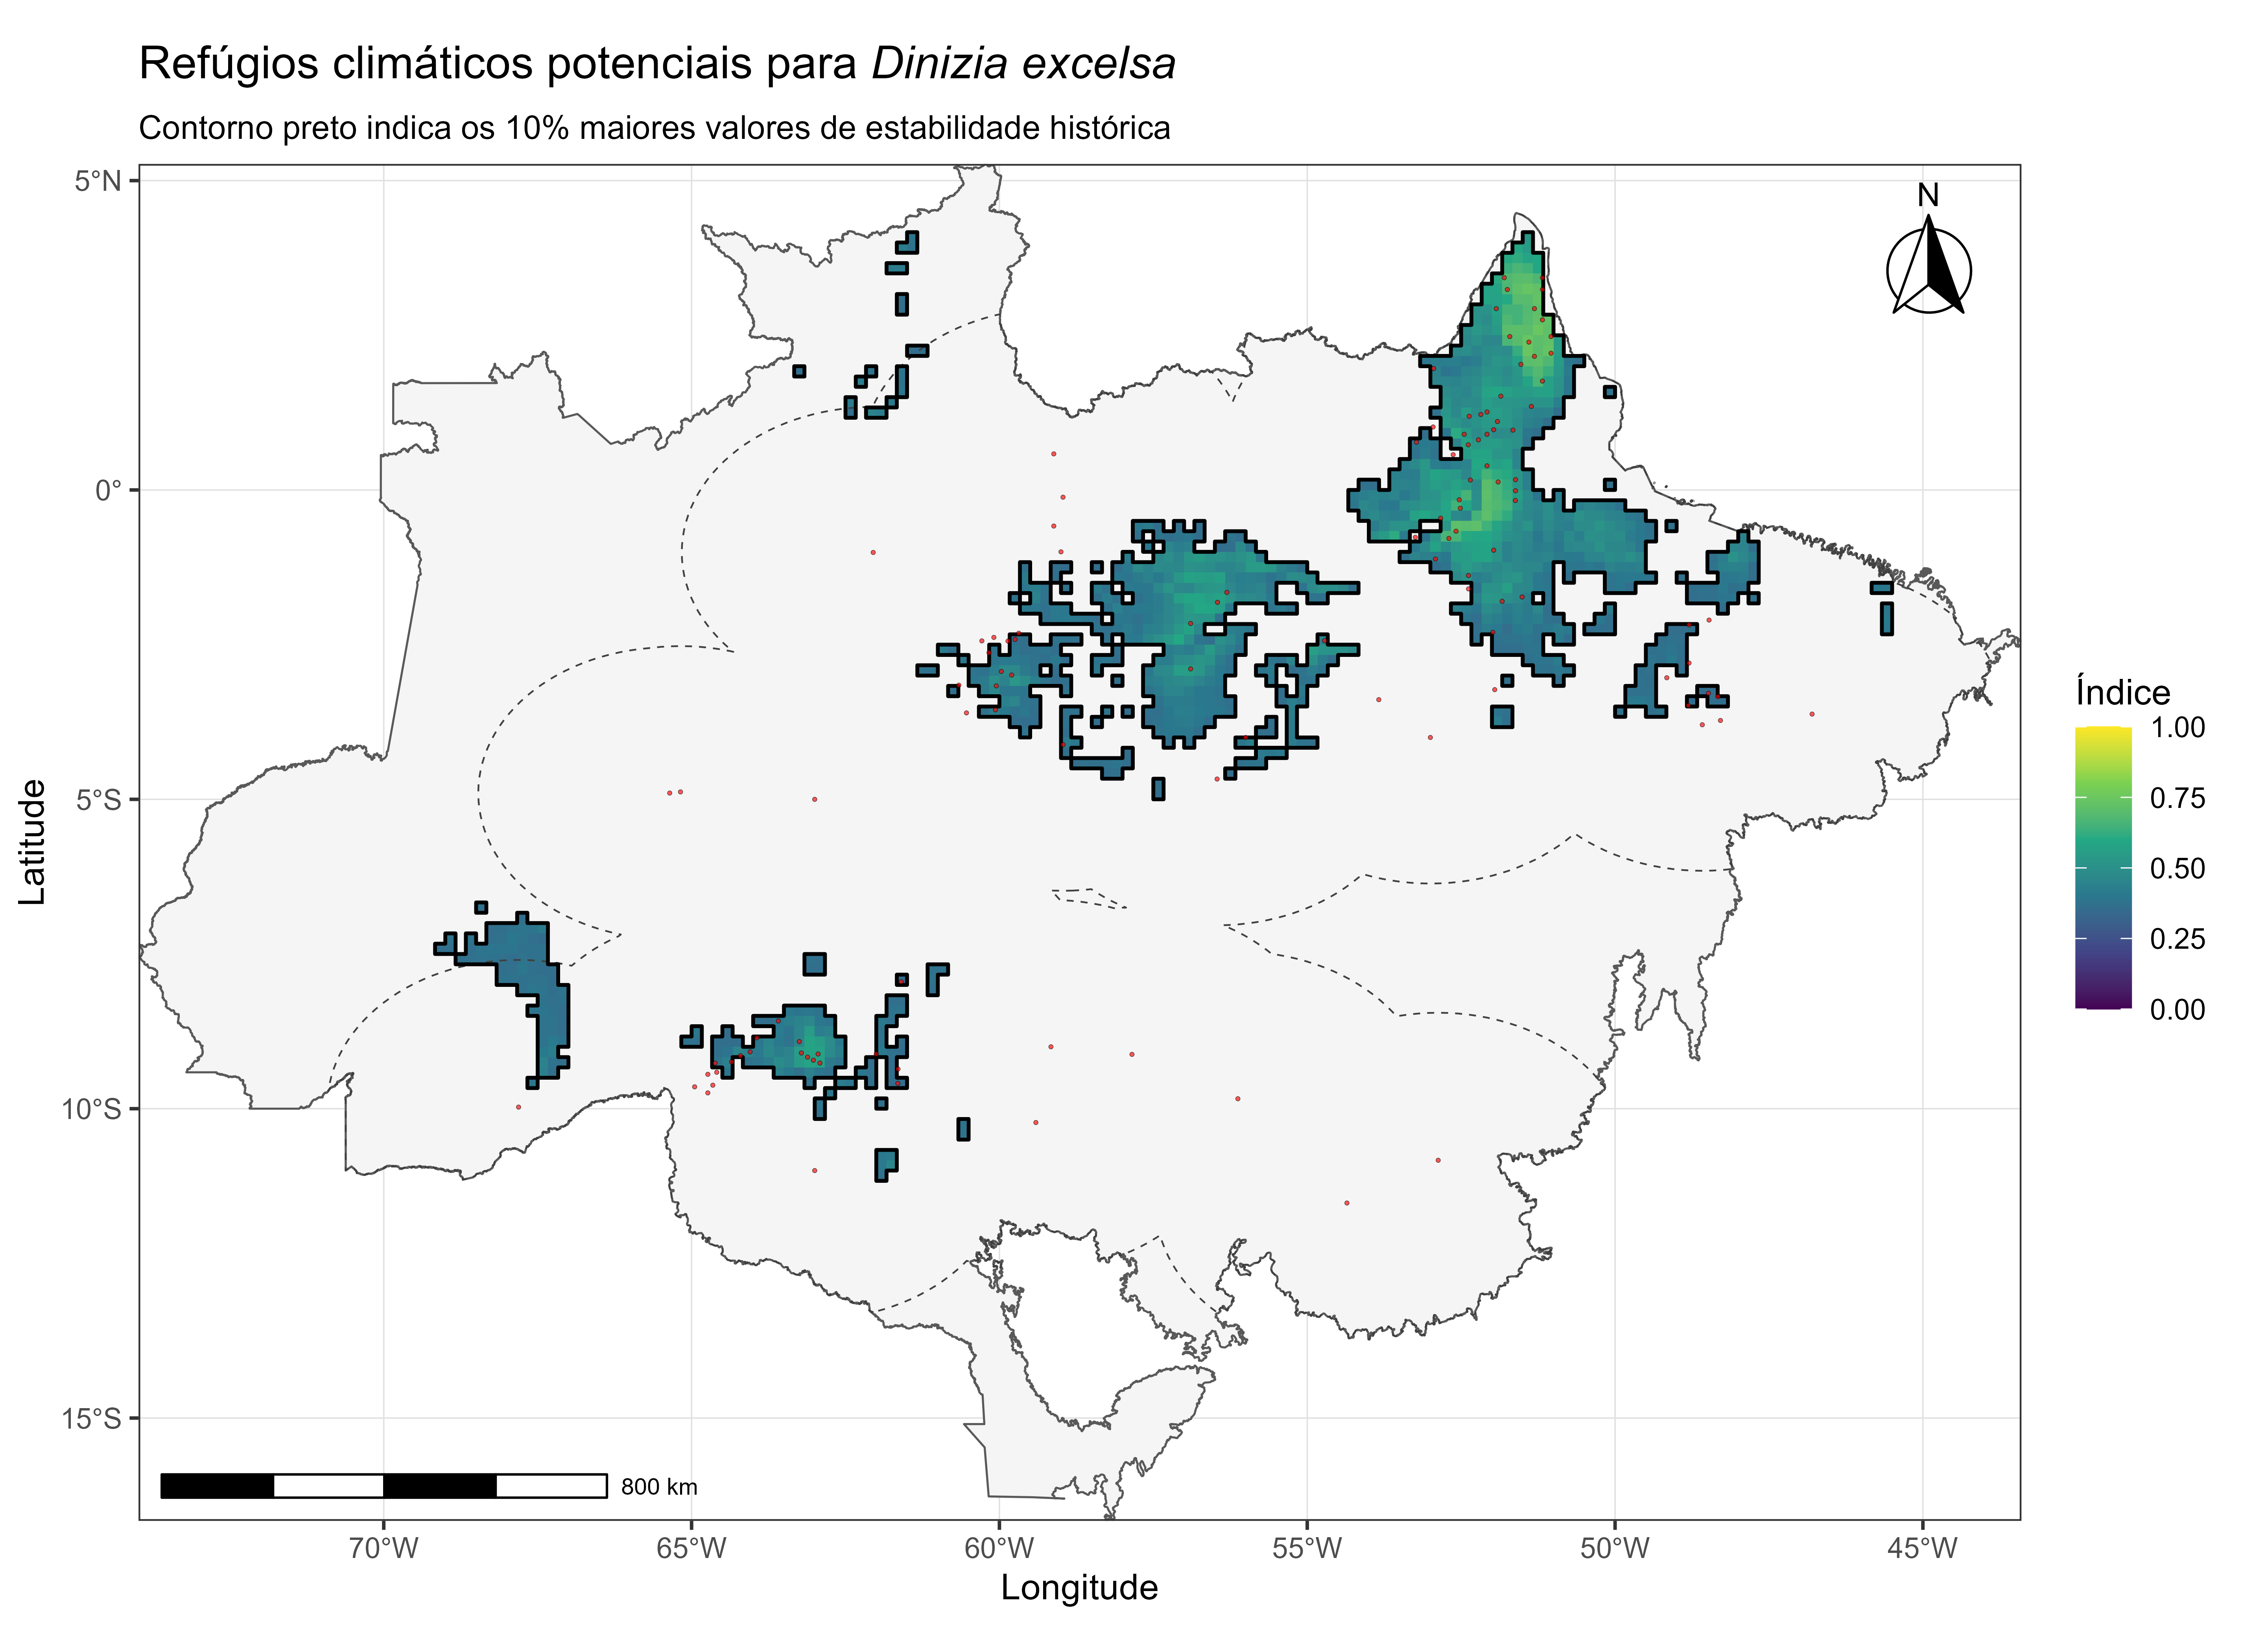
\includegraphics[width=0.96\textwidth]{figuras/unidade17/unidade17_refugios_climaticos.png}
\caption{Candidate areas of long-term climatic suitability for \textit{Dinizia excelsa}, integrating contemporary and paleoclimatic projections.}
\label{fig:unidade17_refugios}
\end{figure}

Persistent modeled suitability identifies climatic-stability candidates, not demonstrated refugia. Conservation claims should be corroborated with phylogeographic, paleoecological, demographic, floristic, or genetic evidence and evaluated against environmental novelty in past projections.

\section{Representation and protection gaps}

\rscriptfile{scripts/unidade17/06_lacunas_protecao.R}

\begin{figure}[H]
\centering
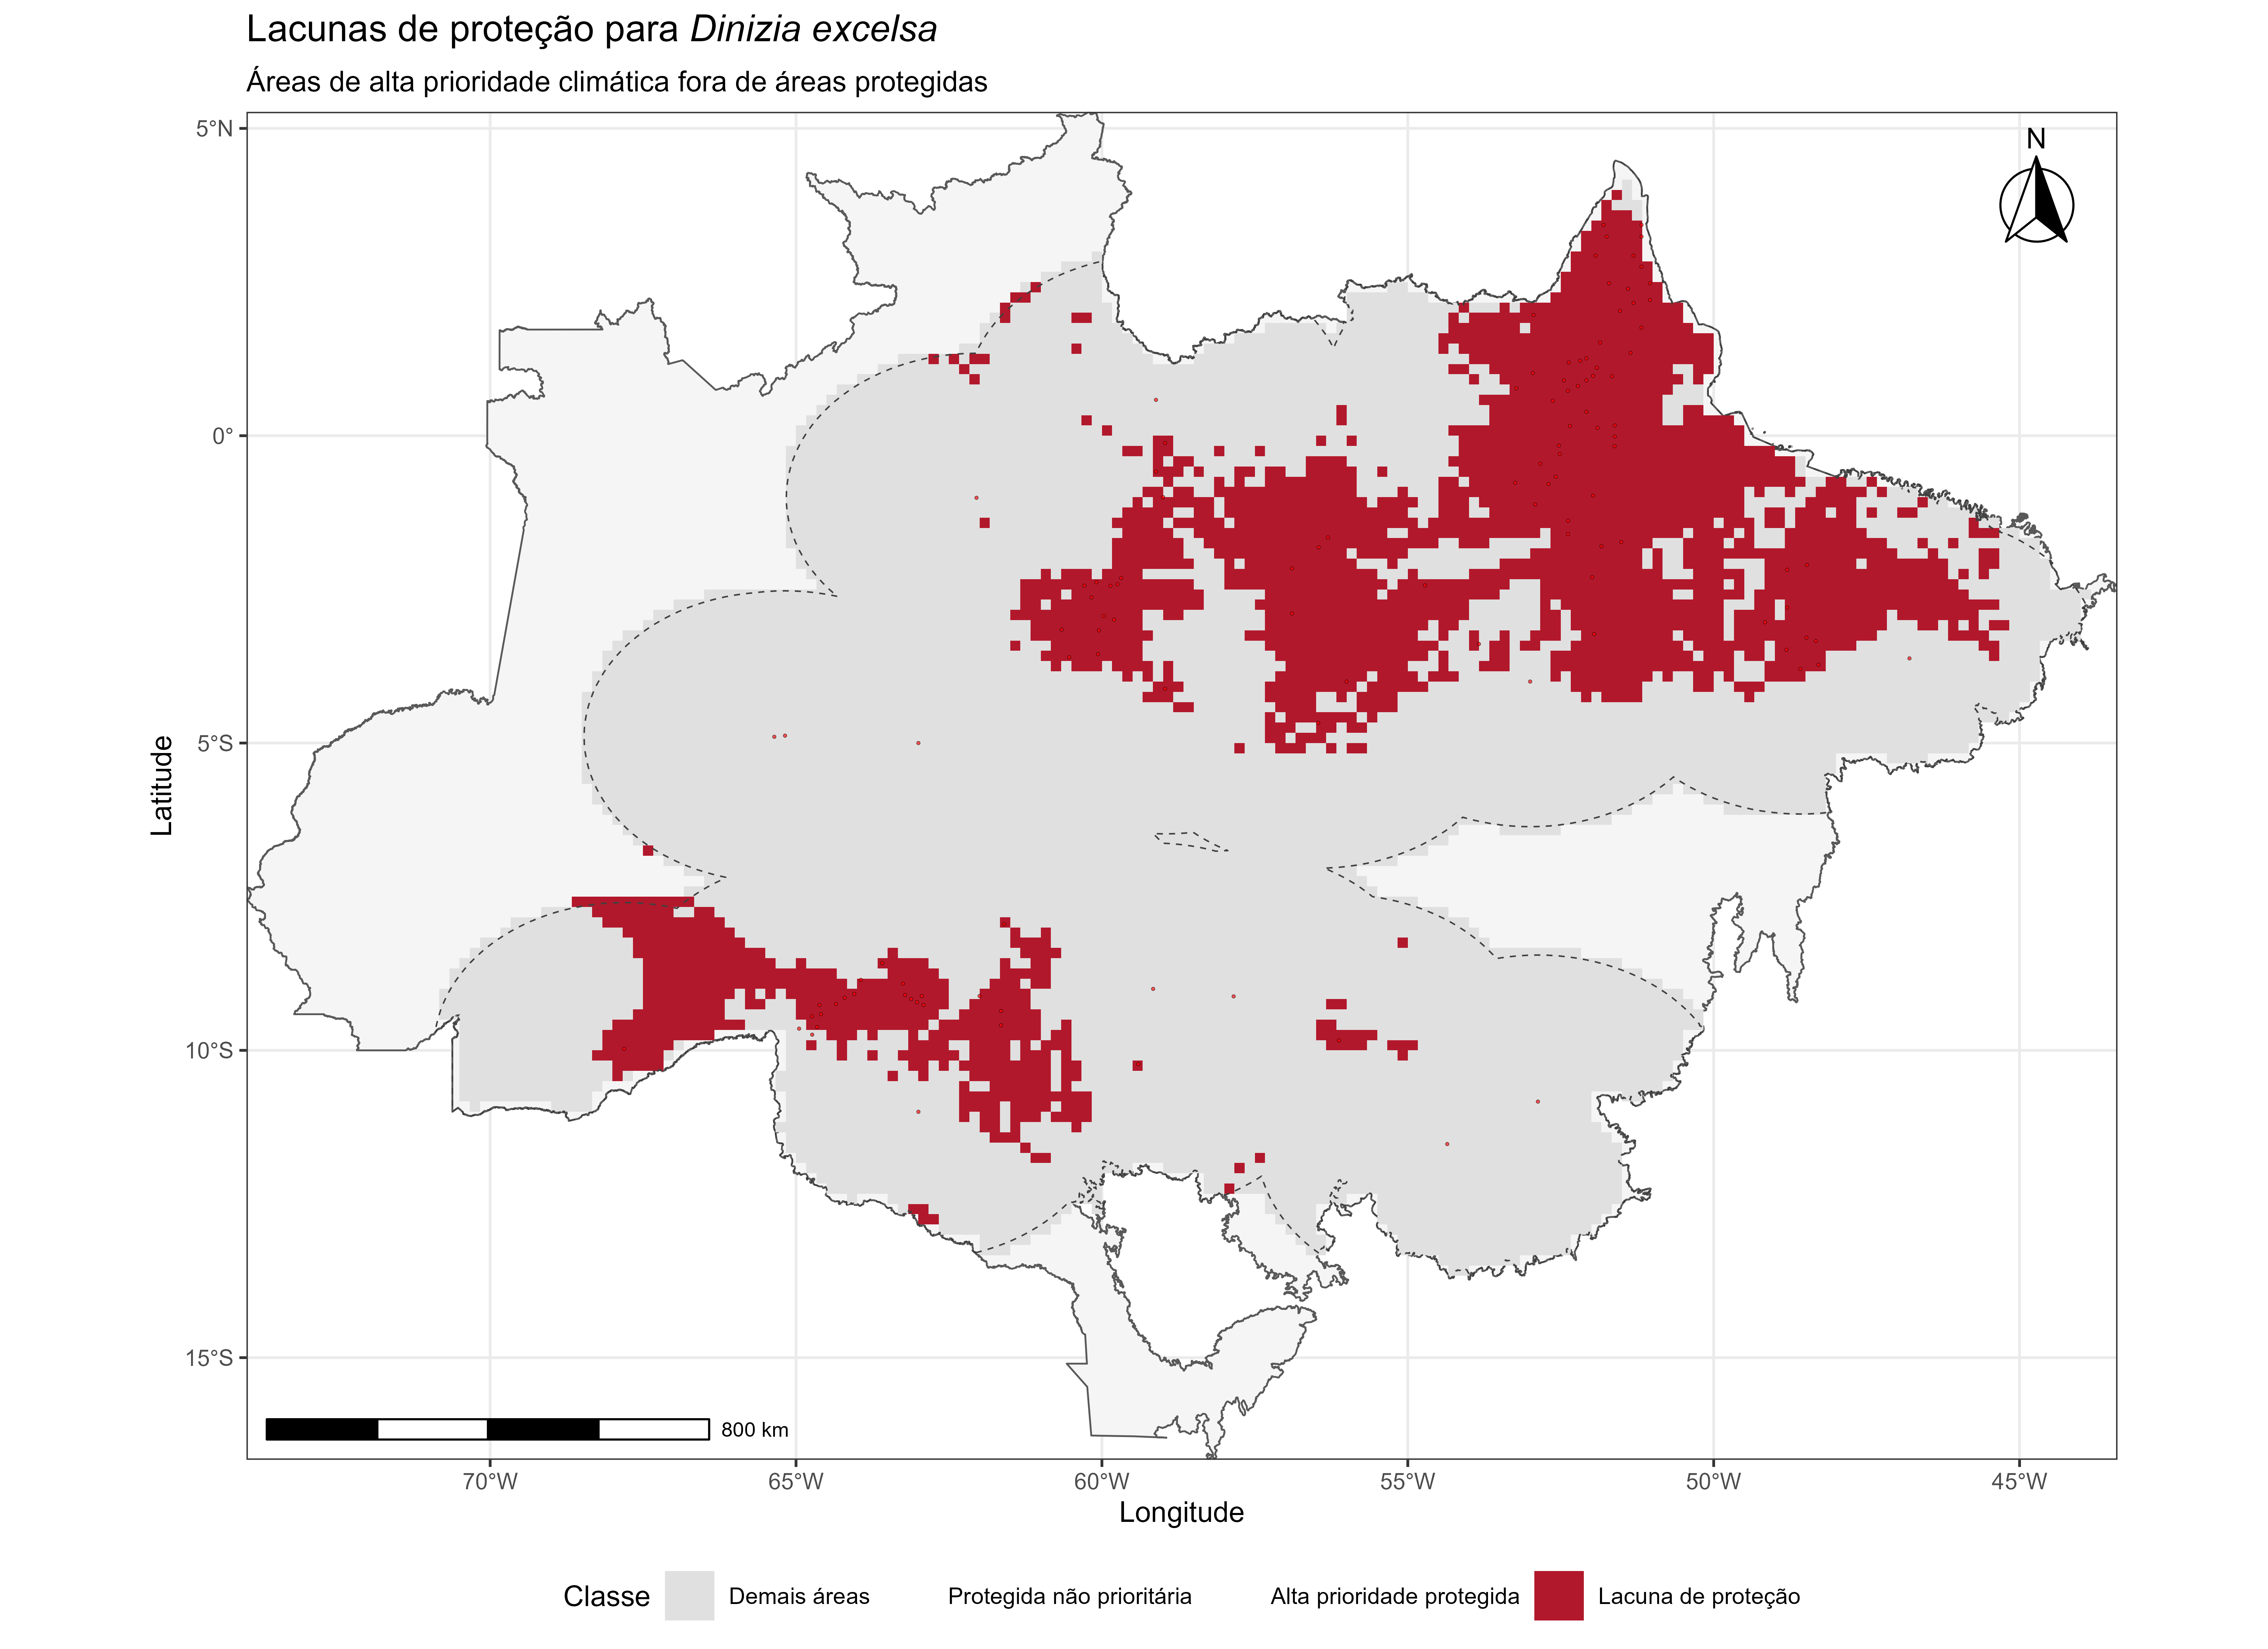
\includegraphics[width=0.90\textwidth]{figuras/unidade17/unidade17_lacunas_protecao.png}
\caption{Potential representation gaps for \textit{Dinizia excelsa}. Candidate priority areas outside the protected-area layer indicate locations requiring further assessment, not automatic proposals for designation.}
\label{fig:unidade17_lacunas}
\end{figure}

A gap analysis should report the fraction and area of each conservation feature represented within the network, ideally stratified by region, environmental class, population unit, and protection category. Nominal coverage is not equivalent to effective conservation: governance, enforcement, land tenure, degradation, and compatible management matter.

\section{An integrated priority index}

\rscriptfile{scripts/unidade17/07_prioridade_integrada_conservacao.R}

\begin{figure}[H]
\centering
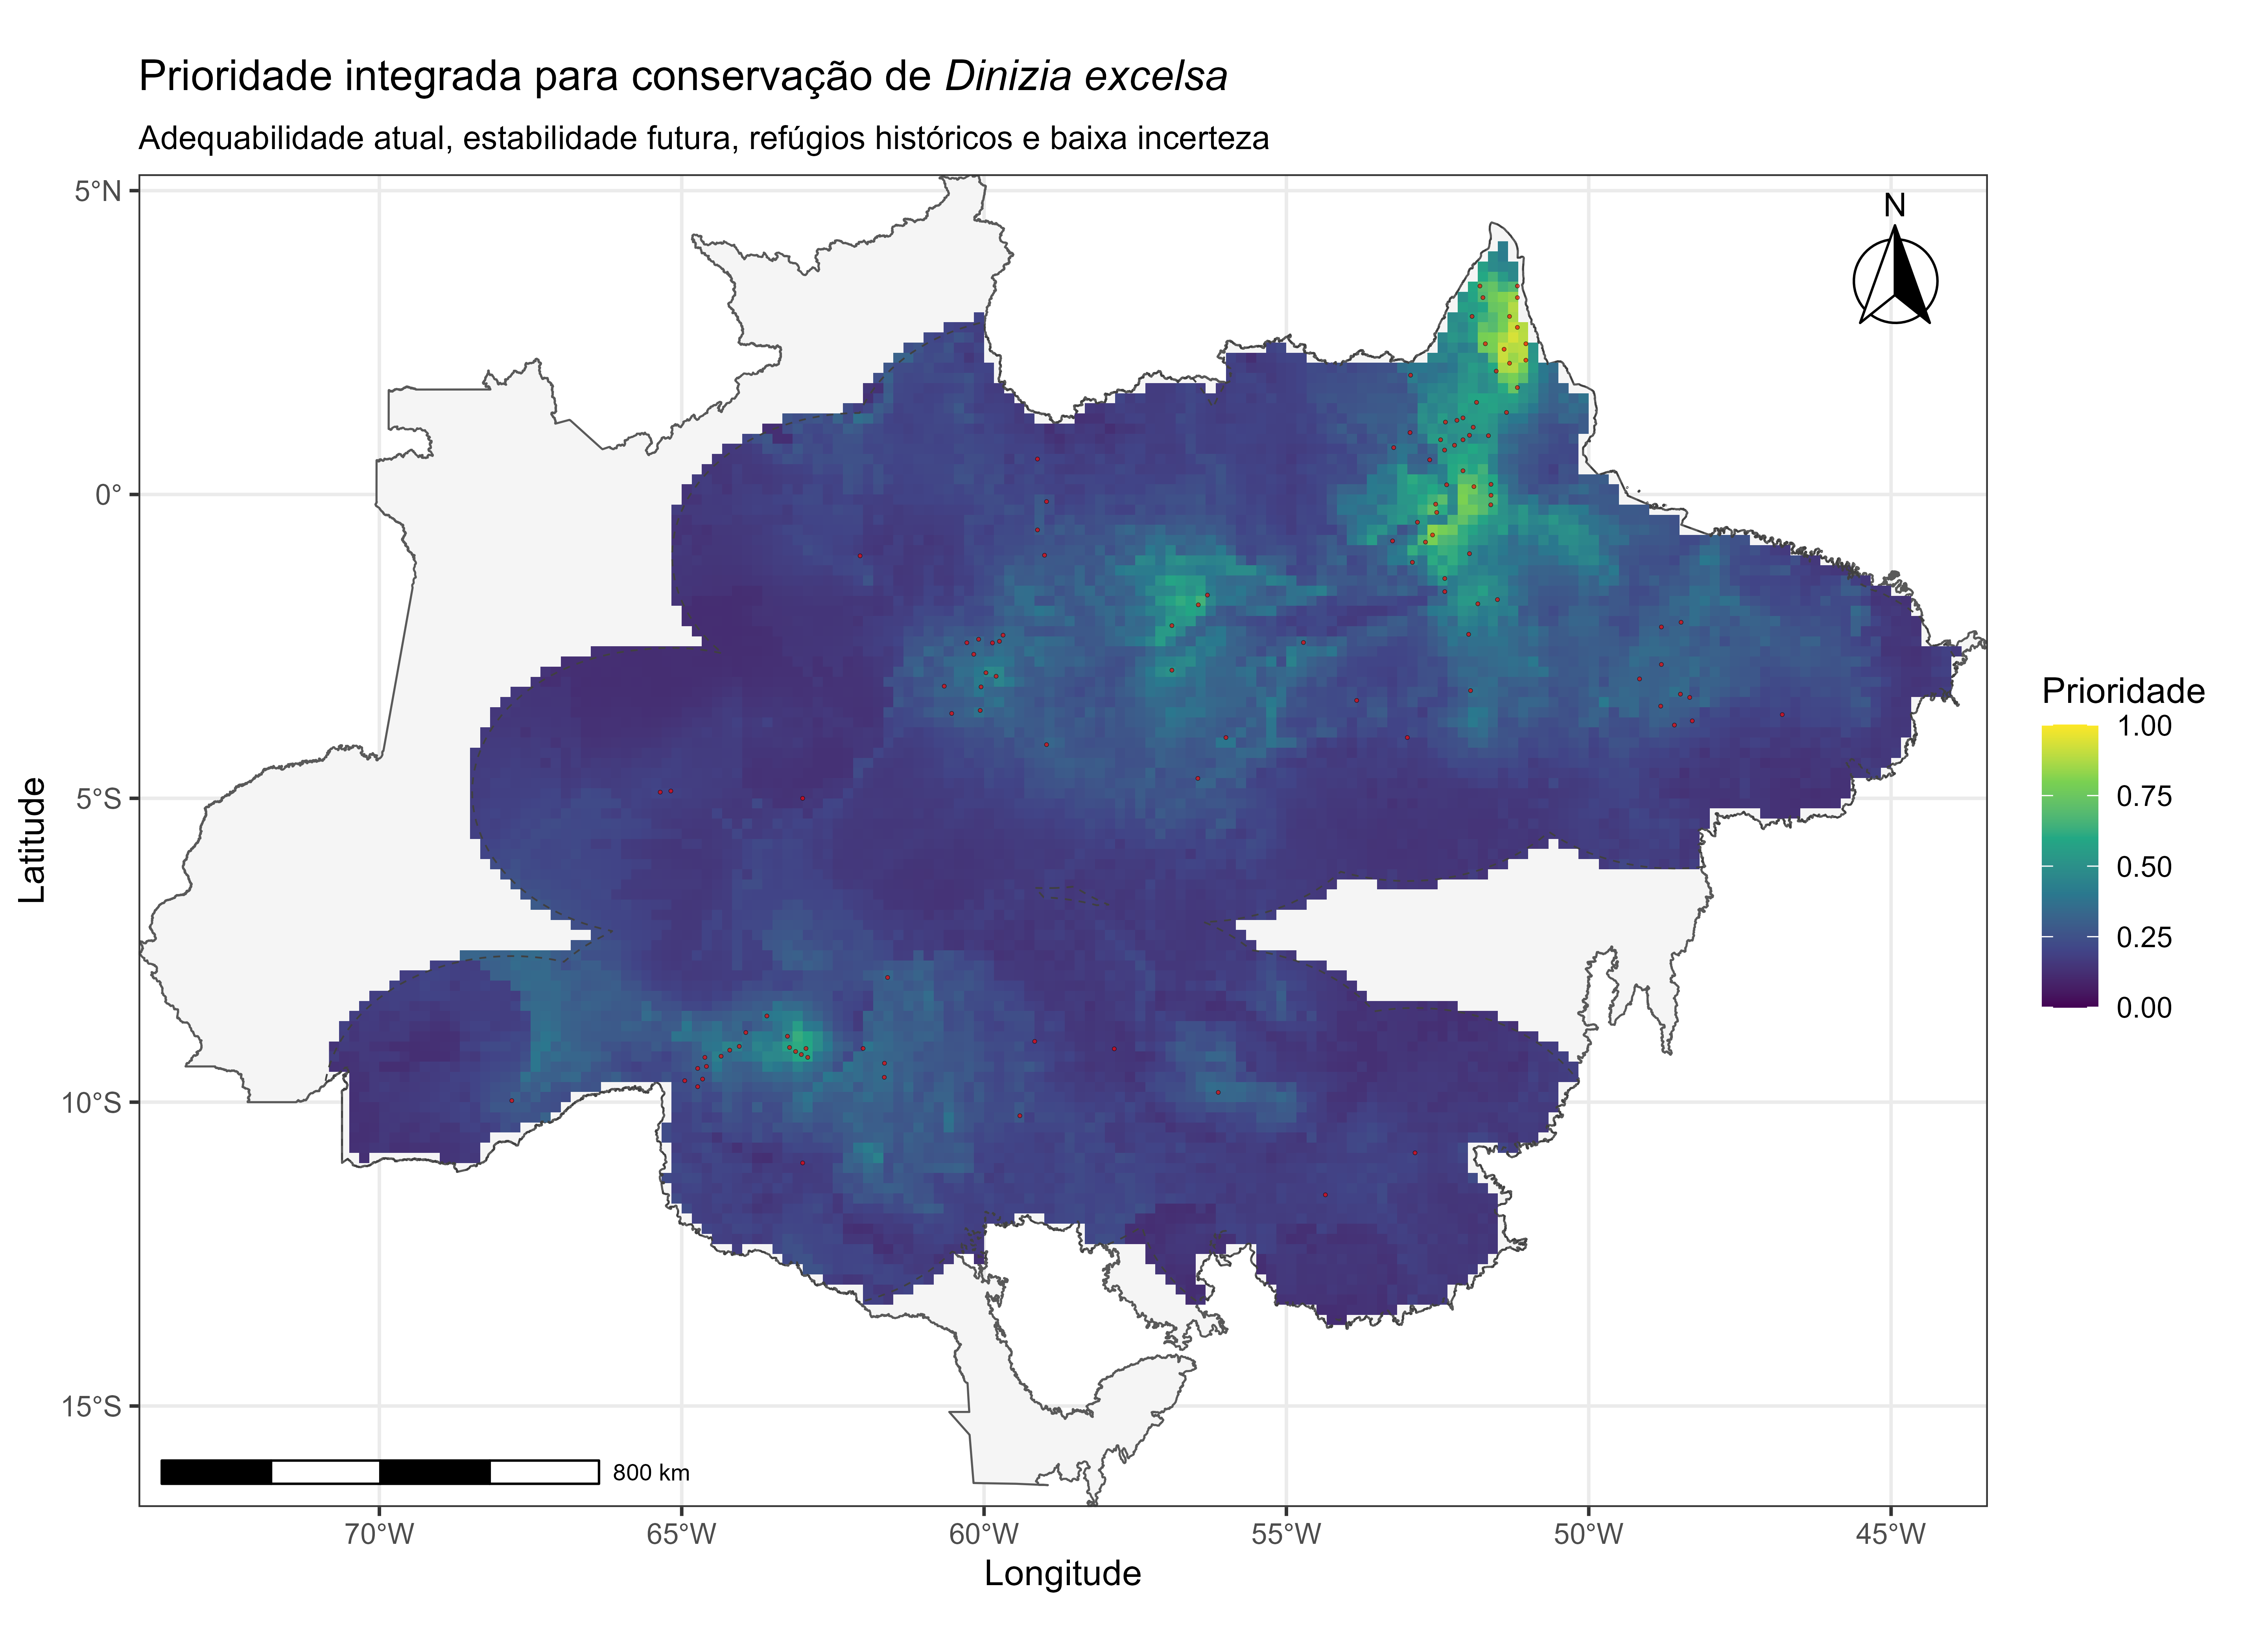
\includegraphics[width=0.90\textwidth]{figuras/unidade17/unidade17_prioridade_integrada.png}
\caption{Integrated screening index for conservation of \textit{Dinizia excelsa}.}
\label{fig:unidade17_prioridade_integrada}
\end{figure}

Weighted overlays are transparent and useful for exploration, but their results depend on normalization, weights, compensation among criteria, and classification cutoffs. A high score in one criterion may offset a critical failure in another unless veto rules are defined. Publish the formula, component layers, weights, rationale, and sensitivity analysis.

For formal systematic conservation planning, cellwise ranking should be replaced or complemented by an optimization framework that represents explicit targets while accounting for cost, complementarity, connectivity, compactness, threats, and existing commitments. Complementarity is crucial: the value of a site depends on what is already protected and on what other selected sites contribute.

\begin{atencao}[title={\faExclamationTriangle\quad A priority index is not an implementation decision}]
The index developed here is a screening tool. Designation, restoration, translocation, or assisted migration requires field verification, feasibility and risk assessment, legal review, stakeholder participation, and consideration of Indigenous Peoples and local communities.
\end{atencao}

\section{Quantitative synthesis}

\rscriptfile{scripts/unidade17/08_sintese_conservacao.R}

\begin{figure}[H]
\centering
\includegraphics[width=0.90\textwidth]{figuras/unidade17/unidade17_sintese_conservacao.png}
\caption{Quantitative summary of screening-priority classes for conservation of \textit{Dinizia excelsa}.}
\label{fig:unidade17_sintese}
\end{figure}

Report continuous scores alongside classes, because areas assigned to categories depend on arbitrary or decision-specific cutoffs. Summaries should state the geographic denominator, pixel-area correction, protected-area version, uncertainty treatment, and sensitivity to alternative criteria and weights.

\section{Complete pipeline}

\rscriptfile{scripts/unidade17/09_pipeline_conservacao.R}

\section{Chapter synthesis}

Applying SDMs to conservation requires integration of ecological modeling, climate change, uncertainty, historical stability, habitat condition, connectivity, and territorial instruments. For \textit{Dinizia excelsa}, this evidence can guide surveys, monitoring, in situ protection, restoration assessment, seed-source planning, and systematic conservation analyses. The maps identify candidates for further evaluation rather than final decisions.

\begin{conceito}[title={\faBook\quad Key message}]
The strongest conservation use of SDM is not simply to locate suitable environments. It is to support an explicit, transparent decision process that represents biodiversity features, maintains persistence and connectivity, acknowledges uncertainty, and accounts for feasibility, costs, and social legitimacy.
\end{conceito}

\section{Review exercises}

\begin{enumerate}
\item How can SDM support conservation of Amazonian tree species without being treated as a map of confirmed occurrence?
\item Why may high suitability and low model disagreement still be insufficient for prioritization?
\item Distinguish a representation gap from ineffective protection.
\item How can future projections change conservation priorities, and how should scenario disagreement be handled?
\item Why does modeled paleoclimatic stability provide only a hypothesis of refugial persistence?
\item How do complementarity and connectivity alter a cell-by-cell suitability ranking?
\item What safeguards are necessary before SDM products inform public conservation decisions?
\end{enumerate}

\section{Synthesis of the applied workflow}

The central lesson of this book is that species distribution modeling is not merely the fitting of algorithms. It is an inferential workflow connecting ecological theory, data quality, biogeographic hypotheses, environmental predictors, calibration design, statistical evaluation, spatial interpretation, transferability, uncertainty, and conservation decisions.

\begin{conceito}[title={\faBook\quad Final applied message}]
A strong SDM is not defined by a high AUC alone. It is built from fit-for-purpose data, explicit hypotheses, a justified calibration domain, ecologically defensible predictors, independently evaluated models, transparent uncertainty, and an interpretation aligned with the scientific or conservation decision.
\end{conceito}

\section{Integrative exercises}

\begin{enumerate}
\item Describe the complete workflow of an SDM project, from occurrence records to a conservation decision.
\item Why does the accessible area \(M\) influence calibration, evaluation, transfer, and conservation interpretation?
\item Compare the roles of GLM, GAM, Random Forest, BRT, and Maxent in an ensemble.
\item Why should component uncertainty and novelty maps accompany final suitability maps?
\item How can future projections support conservation while avoiding deterministic claims?
\item Which data, code, metadata, diagnostics, and decision assumptions should be delivered in a reproducible SDM project?
\item Design an SDM-based conservation study for an Amazonian species, including objectives, targets, costs, validation, uncertainty, and stakeholder participation.
\end{enumerate}

